\documentclass{article}

\usepackage[margin=1in]{geometry}
\usepackage{fancyhdr}
\usepackage{graphicx}
\usepackage{hyperref}
\usepackage{amsmath}
\usepackage{color}
\usepackage{verbatim}

\usepackage{xspace}

\usepackage[margin=1in]{geometry}
\usepackage{listings}
\lstset{language=XML}
\lstset{% general command to set parameter(s)
basicstyle=\footnotesize, % print whole listing small
%basicstyle=\footnotesize, % print whole listing small
keywordstyle=\color{blue}, %\bfseries\underbar,
% underlined bold black keywords
identifierstyle=, % nothing happens
commentstyle=\color{OliveGreen}, % white comments
stringstyle=\ttfamily, % typewriter type for strings
showstringspaces=false, % no special string spaces
language=matlab,
frame=lines,
float=tbfh}

\definecolor{INCFBlue}{rgb}{0.0,0.59,1.0}

\definecolor{issuecolor}{rgb}{0.8,0.8,0.8}
\definecolor{light-gray}{gray}{0.95}
\newcommand{\issue}[1]{%
\begin{center}
\colorbox{issuecolor}{\parbox{0.8\linewidth}{\textbf{Issue:} #1}}
\end{center}%
}

\newcommand{\note}[1]{%
\begin{center}
\colorbox{issuecolor}{\parbox{0.8\linewidth}{\textbf{Note:} #1}}
\end{center}%
}

\newcommand{\suggestion}[2]{%
\begin{center}
\colorbox{issuecolor}{\parbox{0.8\linewidth}{\textbf{#1:} #2}}
\end{center}%
}

\newcommand{\nmlClass}[1]{{\bf #1}}

\newcommand{\ComponentClass}{{\bf{ComponentClass}}\xspace}
\newcommand{\ComponentClasses}{{\bf{ComponentClass}}es\xspace}

\newcommand{\Dynamics}{{\bf{Dynamics}}\xspace}
\newcommand{\Dynamic}{{\bf{Dynamic}}\xspace}

\newcommand{\MathInline}{\tt{Dynamics}}


\newcommand{\Interface}{{\bf{Interface}}\xspace}
\newcommand{\Interfaces}{{\bf{Interface}}s\xspace}


\newcommand{\StateVariable}{{\bf{StateVariable}}\xspace}
\newcommand{\StateVariables}{{\bf{StateVariable}}s\xspace}


\newcommand{\StateAssignment}{{\bf{StateAssignment}}\xspace}
\newcommand{\StateAssignments}{{\bf{StateAssignment}}s\xspace}


\newcommand{\TimeDerivative}{{\bf{TimeDerivative}}\xspace}
\newcommand{\TimeDerivatives}{{\bf{TimeDerivative}}s\xspace}

\newcommand{\Alias}{{\bf{Alias}}\xspace}
\newcommand{\Aliases}{{\bf{Alias}}es\xspace}

\newcommand{\AnalogPort}{{\bf{AnalogPort}}\xspace}
\newcommand{\AnalogPorts}{{\bf{AnalogPort}}s\xspace}

\newcommand{\EventPort}{{\bf{EventPort}}\xspace}
\newcommand{\EventPorts}{{\bf{EventPort}}s\xspace}

\newcommand{\Port}{{\bf{Port}}\xspace}
\newcommand{\Ports}{{\bf{Port}}s\xspace}

\newcommand{\Event}{{\bf{Event}}\xspace}
\newcommand{\Events}{{\bf{Event}}s\xspace}

\newcommand{\Regime}{{\bf{Regime}}\xspace}
\newcommand{\Regimes}{{\bf{Regime}}s\xspace}

\newcommand{\Transition}{{\bf{Transition}}\xspace}
\newcommand{\Transitions}{{\bf{Transition}}s\xspace}

\newcommand{\Trigger}{\tt{Trigger}}

\newcommand{\OnEvent}{{\bf{OnEvent}}\xspace}
\newcommand{\OnEvents}{{\bf{OnEvent}}s\xspace}

\newcommand{\OnCondition}{{\bf{OnCondition}}\xspace}
\newcommand{\OnConditions}{{\bf{OnCondition}}s\xspace}


\newcommand{\Parameter}{{\bf{Parameter}}\xspace}
\newcommand{\Parameters}{{\bf{Parameter}}s\xspace}


\newcommand{\OutputEvent}{{\bf{OutputEvent}}\xspace}
\newcommand{\OutputEvents}{{\bf{OutputEvent}}s\xspace}


\newcommand{\SendPort}{{\tt{SendPort}}\xspace}
\newcommand{\RecvPort}{{\tt{RecvPort}}\xspace}
\newcommand{\ReducePort}{{\tt{ReducePort}}\xspace}
\newcommand{\SendPorts}{{\tt{SendPorts}}\xspace}
\newcommand{\RecvPorts}{{\tt{RecvPorts}}\xspace}
\newcommand{\ReducePorts}{{\tt{ReducePorts}}\xspace}

\begin{document}

\pagestyle{empty}

\begin{center}
{
\includegraphics[width=0.7\columnwidth]{figures/incf_new.png}}

\end{center}

\vspace*{1cm}

\noindent\rule{\columnwidth}{1pt}
\noindent\rule{\columnwidth}{2pt}

\vspace*{1cm}

\begin{center}
\noindent{\Huge \bf Network Interchange for Neuroscience Modeling Language
(NineML)}\\
\vspace{0.5cm}
\noindent{\Large \bf Specification}\\
\vspace{0.5cm}
\noindent{\large INCF Task Force on Multi-Scale Modeling}\\
\vspace{0.5cm}
\noindent{\large Version: 0.1}
\end{center}

\vspace*{0.75cm}

\noindent\rule{\columnwidth}{2pt}
\noindent\rule{\columnwidth}{1pt}

\vspace*{2cm}
\noindent{\Large

{\bf Editors: }
\noindent
\begin{itemize}
\begin{small}
\item Anatoli Gorchetchnikov
\item Ivan Raikov
\item Mike Hull
\item Yann Le Franc
\end{small}
\end{itemize}


\begin{footnotesize}
\noindent Acknowledgments: We would like to thank the Task Force members for their
comments on this document and in particular\\P. Gleeson, E. Muller, A. Davison,
R. Cannon, Birgit Kriener, Subhasis Ray and S. Hill.
\end{footnotesize}

\vspace*{0.3cm}

\noindent
\begin{Large}
This document is under the Common Creative license BY-NC-SA:

\noindent
http://creativecommons.org/licenses/by-nc-sa/3.0/
\end{Large}

\vspace*{0.3cm}

{\flushright 
\includegraphics[width=3cm]{figures/by-nc-sa.png}}

\vspace*{0.3cm}

\noindent {\bf Date:} \today

}

\title{NineML (9ML) Specification}

\newpage
\pagestyle{plain}

\newpage

\abstract

NineML is a simulator independent language with the aim of providing an
unambiguous description of neuronal network models for efficient model sharing
and reusability. This language emerges from a joint effort from experts in the
field of Computational Neuroscience, simulator development and
simulator-independent language initiatives (NeuroML, PyNN), coordinated and
supported by International Neuroinformatics Coordinating Facility (INCF).

This document provides the basis for understanding the Common Object
Model, shared by the three NineML implementations, and the resulting XML
schema and tags. The current work only covers the representation of
spiking neurons and synapses and will be further extended to represent
network connectivity, synaptic plasticity, and all other necessary
concepts to represent networks.  These extensions are still work in
progress and your comments and feedbacks will be extremely valuable.

\newpage
\tableofcontents

\newpage

\section{Introduction}

The increasing number of studies related to neuronal network modeling
and the diversity of the simulation platforms and implementations
cause a major issue for model sharing, replicability and reusability
of either complete models or parts of models. To overcome this problem,
we are proposing a
common description language to be used for exchanging models and being
able to simulate them in any simulation platform.

This description language, using the XML technology, is based on a
common Object Model describing the different elements of network
models. This work, initiated and supported by the International
Neuroinformatics Coordinating Facility as part of the Multiscale
Program, involve Computational Neuroscientists, simulator developers and
developers of simulator-independent language (NeuroML, PyNN).  The name of the
proposed language is NineML (Network Interchange for Neuroscience Modeling
Language).

\subsection{Scope}

The purpose of NineML is to provide a computer language for
succinct and unambiguous description of computational neuroscience models of
spiking neurons networks.

NineML is intended to describe the network architecture, parameters
and equations that govern the dynamics of a spiking neurons network, without
taking into account model implementation detail such as numerical integration
method.

At the current stage of development, the following concepts of spiking neuron
network modeling can be fully or partially described:

\begin{enumerate}
\item spiking neurons
\item synapses
\begin{enumerate}
\item Post-synaptic membrane current mechanisms
\item Short-term synaptic dynamics (a la Markram et. al. 1998)
\item Long-term synaptic modifications (STDP, learning, etc.)
\end{enumerate}
\end{enumerate}

The developed Object Model has been used to create three different
implementations (Java, Python and Chicken Scheme) that are now able to
import/export a common XML description and generate code for simulating the
described model in different simulator.

\subsection{Design Considerations}

As one of the goals of NineML is to provide a mean to import/export a model from
any simulator or implementation, it is crucial to maintain a clear distinction
between the definition of NineML and a simulator. Therefore, NineML should
provide only the information necessary for any given simulator
to instantiate the network models in a simulator agnostic way.
For example, NineML should specify the neuron membrane equation to solve,
but not how to solve it.  In addition, for implementation and performance
reasons, it is important to keep the language layer ``close'' to the simulator
-- such that the language layer is not responsible for maintaining separate
representations of all the instantiated elements in the network.

A NineML object model representation can take multiple forms.  A
program can employ a concrete representation of the NineML objects in
a specific programming language, or it can convert an internal model
representation to and from the NineML XML schema, or it can take the
form of an interpreter for the NineML native language as a compact
representation and use code generation to produce a model
representation for a target simulation environment.

It is important to note that the NineML XML schema is isomorphic to the NineML
object model.

The design of NineML is divided into two semantic layers:
\begin {enumerate}
\item An {\bf Abstraction Layer} that provides the core concepts and
mathematical descriptions with which model variables and state update
rules are explicitly described in {\em parametrized} form, and
\item A {\bf User Layer} that provides a syntax to specify the
instantiation and the value of parameters of all these components of a network
model.
\end {enumerate}

As the User Layer provides the mechanism for instantiating and
parametrization of the model elements that have been defined in the
Abstraction Layer, it is clearly essential that these two layers share
a complementary and compatible design philosophy. There is a
clear definition of which aspects of a model are defined in the User
Layer and which are defined in the Abstraction Layer. In addition,
the mechanisms for naming and addressing Abstraction Layer concepts
that are instantiated in the User Layer have been kept simple for the
user.

\subsection{About this document}

This document presents the current NineML specifications and consists of:
\begin{enumerate}
\item a description of the Abstraction and User Layer Object models
\item the XML serialization with the description of the different tags
\item documented examples of XML descriptions
\item a proposal to solve the transition resolution problem
\end{enumerate}

\section{Units and Dimensions in NineML}
\label{dimensions}

\noindent
Each specification of a parameter or a state variable in the definition of
a class of component must state its dimension. A dimension declaration
associates a name with values for the powers for each of seven SI base
units: length, l; mass, m; time t; electric current i; temperature T;
luminous intensity L and amount of substance, n.
For example, acceleration has dimension $lt^{-2}$ and voltage is
$ml^2t^3i^{-1}$.
Dimensions can be declared at the top level of a NineML file with
the "Dimension" element with attributes for each of the base dimensions or
imported from a specific XML file, describing a set of dimensions.

Each dimension can give rise to a family of unit declarations, each of
which has the same dimensionality but a different multiplier. For example,
typical units for a quantity with dimensionality voltage include
milliVolts (multiplier = $10^{-3}$), microVolts (multiplier = $10^{-6}$)
and Volts (multiplier = 1).  To express a dimensional quantity both a
numerical factor and a unit are required. Units can be expressed in a NineML
file with the "unit" element, defined at the User Layer level or imported
from a specific XML file, describing a set of units.

Except where physical constants are required, abstraction layer definitions
generally only contain references to dimensions and are independent of any
particular choice of units. Conversely, the user layer only refers to units.
Internally, dimensional quantities are to be understood
as rich types with a numerical factor and exponents for each of the
base dimensions. They are independent of the particular choice of
units by which they are assigned.

\section{Abstraction Layer: Core Concepts }
\label{AbstractionL}

The Abstraction Layer aims at providing general concepts to represent the
mathematical entities (functions, differential equations, event handling,...)
defining the dynamics of the different types of models composing a network
(neuron models, synapse models, synaptic/intrinsic
plasticity, ...)

\subsection{ComponentClass}


\begin{table}[htb]
\center
\begin{tabular}{|c|}
\hline
\hline
ComponentClass \\
\hline \\
\colorbox{issuecolor}{\parbox{0.4\linewidth}
{\center {\tt Dynamics} object}} \\
\hline
\colorbox{issuecolor}{\parbox{0.4\linewidth}
{\center {\tt Interface} object}} \\
\hline
\end{tabular}
\end{table}


The main building block of the Object Model is the \ComponentClass.
The \ComponentClass object is intended to package together a collection of
objects that relate to the definition of a model (cells, synapses, synaptic
plasticity rules, random spike trains, inputs, ...).
All equations and event declarations that are part of particular entity
model, such as neuron model for instance, belong in a single \ComponentClass.
A \ComponentClass can be used to represent either a specific model of neuron or a
composite model, including synaptic mechanisms (as in the second example
provided in the Appendix for example) as long as the algebra is correct.
A \ComponentClass is composed of a \Dynamics block and \Interfaces, as shown
in Figure~\ref{fig:EX1_RegimeGraph}. The \Dynamic block represent the internal
dynamic of the model while the \Interface block allows the \ComponentClass to
communicate with other instantiations of the \ComponentClass and with the User
Layer.

\begin{figure}[htb!]
\center
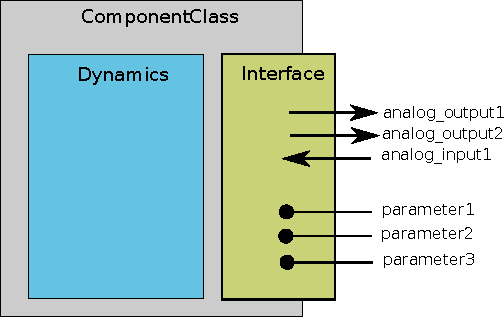
\includegraphics[width=8cm]{figures/component_simple.pdf}
\protect\caption{ComponentClass Overview (Simple)}
\label{fig:EX1_RegimeGraph}
\end{figure}

\subsection{Dynamics}


\begin{table}[htb]
\center
\begin{tabular}{|c|}
\hline
\hline
Dynamics \\
\hline \\
\colorbox{issuecolor}{\parbox{0.4\linewidth}
{\center Set of {\tt StateVariable} objects}} \\
\hline
\colorbox{issuecolor}{\parbox{0.4\linewidth}
{\center Set of {\tt Regime} objects}} \\
\hline
\colorbox{issuecolor}{\parbox{0.4\linewidth}
{\center Set of {\tt Alias} objects}} \\
\hline
\end{tabular}
\end{table}


The \Dynamics block represents the \emph{internal} mechanisms
governing the behaviour of the component.  For most of the models
these dynamics are non-linear, presenting transitions between
different regimes at particular values of one or different \StateVariables.
To create a representation that include both simple
dynamics and non-linear dynamics, the \Dynamics block can contains the
following concepts:

\begin{itemize}
\item \StateVariable (section~\ref{state-var})
\item \Regime (section~\ref{regime}) that describe the dynamics of the
system for a particular domain of \StateVariable
\item \Transition (section~\ref{transition}) that links two
regimes: the Source \Regime and the Target \Regime, and can be triggered by
an event or a condition. If a component is in the Source \Regime, and the
transition is triggered, then the component moves into the Target \Regime.
\item \Alias (section~\ref{alias})
\end{itemize}


These different concepts are the building blocks of a graph, called
the {\tt Regime Graph} (illustrated in Figure~\ref{SimpleRegimeGraph}),
where the \Regime forms the vertices and the \Transition form the
directional edges of the {\tt Regime Graph}. This graph must have at
least one \Regime, and contain no regime islands. At any given time,
a component will be in a single \Regime, and can change which \Regime
it is in through \Transition.

\begin{figure}[htb!]
\center
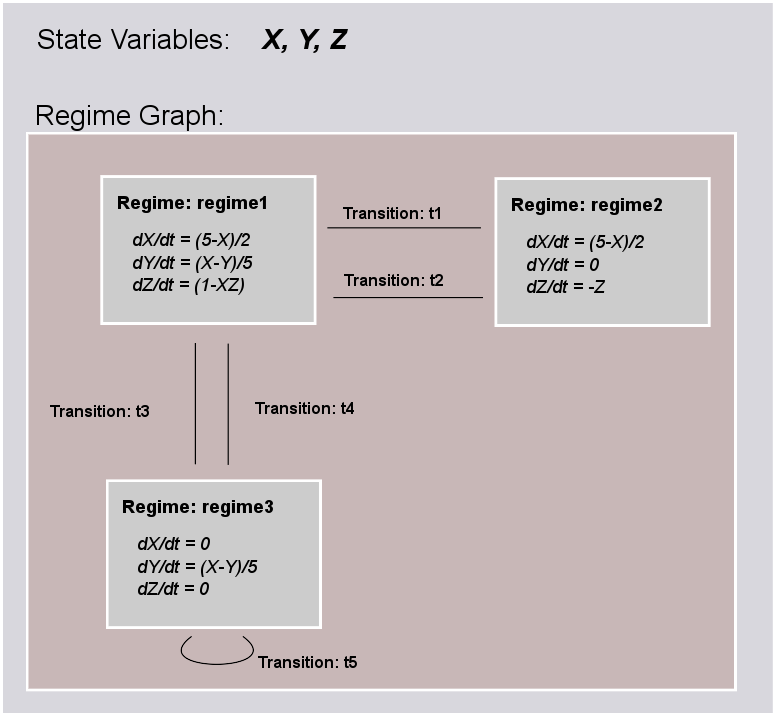
\includegraphics[width=14cm]{images/SimpleRegimeGraph.png}
\protect\caption{The dynamics block for an example component.}
\label{SimpleRegimeGraph}
\end{figure}

An example dynamics in Figure~\ref{SimpleRegimeGraph} has three \StateVariables,
\emph{X,Y} and \emph{Z}, and a state graph with three \Regimes, \emph{regime1},
\emph{regime2} and \emph{regime3}. At any time, a component will be in one of
these regimes, and the state variables will evolve accordingly.

\subsubsection{StateVariable}
\label{state-var}

The internal state of a component is defined by a set of \StateVariable
-- variables that can change either continuously or discontinuously as a
function of time.

\begin{table}[htb]
\center
\begin{tabular}{|c|}
\hline
\hline
StateVariable \\
\hline
\hline
{\em name}: {\tt String} \\
\hline
{\em dimension}: {\tt Dimension} \\
\hline
\end{tabular}
\end{table}

The \StateVariable changes happen in two ways:
%
\begin{quote}
\begin{itemize}
\item continuously through \textbf{TimeDerivatives} (in \Regimes),
which define the \StateVariables evolution over time, for example
$dX/dt=1-X$.
\item discretely through \StateAssignment (in \Transition),
which make discrete changes to a \StateVariable value, for example
$X = X + 1$.
\end{itemize}
\end{quote}

\subsubsection{Regime}
\label{regime}


\begin{table}[htb]
\center
\begin{tabular}{|c|}
\hline
\hline
Regime \\
\hline
\hline
{\em name}: {\tt String} \\
\hline
\colorbox{issuecolor}{\parbox{0.4\linewidth}
{\center Set of {\tt TimeDerivative} objects}} \\
\hline
\colorbox{issuecolor}{\parbox{0.4\linewidth}
{\center Set of {\tt OnCondition} objects}} \\
\hline
\colorbox{issuecolor}{\parbox{0.4\linewidth}
{\center Set of {\tt OnEvent} objects}} \\
\hline
\end{tabular}
\end{table}


A \Regime is defined in NineML as a system of ODEs in time
on \StateVariable.  As such, \Regime defines how the \StateVariables
change (propagate in time) between subsequent \Transitions. \Regime is
defined to have non-vanishing temporal extent. Once construction of
the \Regime is complete, it should have defined the following
properties:

\begin{itemize}
\item An unordered collection of \nmlClass{StateVariable}s which are
propagated when the \nmlClass{Regime} is active.
\item a set of \TimeDerivative, one for each \StateVariable
of the \ComponentClass, which define how the \StateVariable
evolve over time in the form $\frac{dx_{i}}{dt} = f(x\_0, ..., x\_i, t)$.
\item \nmlClass{Parameter}s for the \nmlClass{Regime}
\item An unordered collection of \nmlClass{AnalogPort}s which publish state
variables (type=send), or consume state variables published from elsewhere
(type=recv, or type=reduce).
\item The independent variable must be shared between the collection
of \nmlClass{StateVariable}s and their propagators in a \Regime.
\end{itemize}

\note{If a \nmlClass{TimeDerivative} for a \StateVariable is not defined
in a \Regime, it is assumed to be zero.}

It is important to note that, at the current stage of development, we are only
considering "Temporal regimes". In the future, the concept could be extended
to more general cases where the independent variable can be anything (space
for example)

\subsubsection{OnCondition}

\nmlClass{OnCondition}s are the mathematical expressions which define
when a \nmlClass{Transition} should be triggered.
\nmlClass{OnCondition}s are any arbitrary combination of \emph{Logical
Operations} (and, or, noop, etc.) on the
result of any arbitrary combination of \emph{Relational Operations}
($>$,$<$,$==$,$<=$,$>=$, etc.) on
\nmlClass{StateVariable}s. At any given time in the \nmlClass{Regime},
the \nmlClass{OnCondition} expression then evaluates to True or False
{\tt Boolean} result. For example, the following are valid
\nmlClass{OnCondition}s

\begin{verbatim}
x>10
x>10 & y<20
x>exp(-cos(y)) | y<sin(t)+5
x==15
\end{verbatim}

\begin{table}[htb]
\center
\begin{tabular}{|c|}
\hline
\hline
OnCondition \\
\hline
\hline
{\em trigger}: {\tt Trigger} \\
\hline
\colorbox{issuecolor}{\parbox{0.4\linewidth}
{\center Set of {\tt StateAssignment} objects}} \\
\hline
\colorbox{issuecolor}{\parbox{0.4\linewidth}
{\center Set of {\tt EventOut} objects}} \\
\hline
\end{tabular}
\end{table}

A \nmlClass{OnCondition} which persistently evaluates to True violates
the definition that \nmlClass{Transition}s should have vanishing
temporal extent, and the behaviour for this case is undefined, but it
would be preferable for the implementation to produce an error message
to the user.

\subsubsection{Transition}
\label{transition}

Movement between several instances of \Regime happens via \Transition.
A \nmlClass{Transition} is defined in NineML as having
a source and target \nmlClass{Regime}, where the target
\nmlClass{Regime} can be the same as the source (For example \emph{t5}
in Figure~\ref{SimpleRegimeGraph}). There are two types of \Transition:

\begin{itemize}
\item An \OnCondition function of the \StateVariable, for
example $X > Y$.
\item An \OnEvent on an input from \EventPort. (See section~\ref{port}).
\end{itemize}

\begin{table}[htb]
\center
\begin{tabular}{|c|}
\hline
\hline
Transition \\
\hline
\hline
{\em source}: {\tt Regime} \\
\hline
{\em target}: {\tt Regime} \\
\hline
\end{tabular}
\end{table}

During either type of transition three things can happen:
\begin{itemize}
\item The component can change regime. For example, in figure 2, if
the component is in \emph{regime3}, and the trigger for \emph{t3} is
satisfied, then the component will move into \emph{regime1}.
\item \textbf{StateAssignment}s can take place, for example, $X=0$
\item The component can send \OutputEvent
\end{itemize}

During a transition, multiple \StateAssignment and \OutputEvent can occur.
(For more on the resolution of \nmlClass{Transition}s see Appendix
section~\ref{resolution})

\nmlClass{Transition}s have a vanishing temporal extent (i.e. they are
event-like). Once construction of a \nmlClass{Transition} is complete, it
should have defined the following properties:
\begin{itemize}
\item The \nmlClass{Condition} or \nmlClass{EventPort(mode=recv)} which
triggers the \nmlClass{Transition}
\item A set of \StateAssignment and \OutputEvent objects
\item The label of the source \nmlClass{Regime}, and the label of the target
\nmlClass{Regime}, which may be the same as the source \nmlClass{Regime}.
\end{itemize}

\subsubsection{Aliases}
\label{alias}

An alias corresponds to an intermediate variable allowing to store an
information and to reuse it at different places in the definition of
the dynamics.

\begin{table}[htb]
\center
\begin{tabular}{|c|}
\hline
\hline
Alias \\
\hline
\hline
{\em name}: {\tt String} \\
\hline
{\em rhs}: {\tt MathInline} \\
\hline
\end{tabular}
\end{table}

\textbf{Aliases} are motivated from two problems:

\begin{itemize}
\item {\bf substitution}: rather than writing long expressions for functions of
\StateVariable, we can define an \Alias once. For example, we can define chains
of \Aliases:
%
\begin{quote}{\ttfamily \raggedright \noindent
m\_alpha~=~(alphaA~+~alphaB*V)~/~(~alphaC~+~exp((alphaD+V/alphaE))~)\\
m\_beta~=~~(betaA~+~betaB*V)~/~(~betaC~+~exp((betaD+V/betaE))~)\\
minf~=~m\_alpha~/~(m\_alpha~+~m\_beta)\\
mtau~=~1./(m\_alpha+m\_beta)\\
dm/dt~=~(1/C)~*~(minf-m)/mtau
}
\end{quote}

In this case, $m_{alpha}$, $m_{beta}$, $minf$ and $mtau$ are all
alias definitions. There is no reason we couldn't expand our $dm/dt$
description out to eliminate these intermediate \Aliases, but the expression
would be very long and difficult to read.

\item {\bf Accessing intermediate variable}: if we would like to communicate a
value other than a simple \StateVariable to another \ComponentClass. For
example, if we have a component representing a
neuron, which has an internal \StateVariable, 'V', we may be interested in
transmitting a current, for example $i=g*(E-V)$.

\end{itemize}

\note{\Alias is defined in the Dynamics, \emph{not} in the
\Regime. This means that aliases are the same across all regimes.}

\subsection{Interfaces}

\begin{table}[htb]
\center
\begin{tabular}{|c|}
\hline
\hline
Interface \\
\hline
\colorbox{issuecolor}{\parbox{0.4\linewidth}
{\center Set of {\tt Parameter} objects}} \\
\hline
\colorbox{issuecolor}{\parbox{0.4\linewidth}
{\center Set of {\tt Port} objects}} \\
\hline
\end{tabular}
\end{table}


The interface is the \emph{external} view of the \ComponentClass that defines
what inputs and outputs the component exposes to other \ComponentClasses and the
parameters that can be set for the \ComponentClass. The interface consists of
instances of \Port (section~\ref{port}) and \Parameter
(section~\ref{parameters}).

As well as being able to specify the communication of continuous values,
\ComponentClasses are also able to specify the emission and the reception
of \Events. Events are discrete notifications
that are transmitted over \EventPorts (section~\ref{port}). Since
\EventPorts have names, saying that we transmit `event1' for example
would mean transmitting an event on the EventPort called `event1'. Events
can be used for example to signal action potentials firing.

\subsubsection{Parameter}
\label{parameters}

Parameters correspond to a placeholder for a numerical value with
dimension (this value can also be defined as dimensionless).

\begin{table}[htb]
\center
\begin{tabular}{|c|}
\hline
\hline
Parameter \\
\hline
\hline
{\em name}: {\tt String} \\
\hline
{\em dimension}: {\tt Dimension} \\
\hline
\end{tabular}
\end{table}

It defines particular aspects of the model, such as the firing threshold,
reset voltage, the
decay time constant of a synapse model.  The instantiation of
Parameters at the Abstraction Layer level allow us to define the
dynamics of a general component.  It is then possible to instantiate
several variants of this component by attributing different values for
the \Parameters, in the User Layer.  For example, if we are building
an integrate-and-fire neuron, we can specify that the Reset-Voltage
and the Firing-Threshold are parameters, write our dynamics in terms
of these parameters, then use the User Layer to provide parameters to
create different neurons. By definition, Parameters are set at the
start of the simulation, and remain constant throughout.


\subsubsection{Port}
\label{port}

Ports allow instantiations of \ComponentClasses to communicate between each
other during a simulation.
There are two sub-classes of \nmlClass{Port} objects: \nmlClass{AnalogPort}
and \nmlClass{EventPort}, and each can have different modes.

\paragraph{AnalogPort}


\begin{table}[htb]
\center
\begin{tabular}{|c|}
\hline
\hline
AnalogPort \\
\hline
\hline
{\em name}: {\tt String} \\
\hline
{\em mode}: {\tt PortMode} \\
\hline
{\em dimension}: {\tt Dimension} \\
\hline
{\em reduce\_op}: {\tt ArithOp} option \\
\hline
\end{tabular}
\end{table}


AnalogPorts transmit and receive continuous values, either \Alias
or \StateVariable. \AnalogPort can have 3 modes:
\begin{itemize}
\item \SendPort - transmit data originating in this \ComponentClass which can
be read by other \ComponentClasses.
\item \RecvPort - receive data from another \ComponentClasses \SendPort
port. Each \RecvPort can be connected to \emph{one} \SendPort.
\item \ReducePort - receive data from multiple \SendPorts. These
differ from \RecvPorts in that they can be connected to multiple
\SendPort. \ReducePorts take an additional operator,
{\tt reduce\_op}, which specifies how the data from multiple \SendPorts
should be combined to produce a single value. Currently, the
only supported operations is $+$, which sums the inputs.
The motivation for \ReducePort is that it allows us to make our
\ComponentClass definitions more general. For example, if we are defining a
neuron, would define a \ReducePort called {\tt InjectedCurrent}.
This allows us to write the membrane equation for that neuron as
$dV/dt = (1/C) * InjectedCurrents$.

Then, when we connect this neuron to synapses, current-clamps, etc, we
simply need to connect the SendPorts containing the currents of these
\ComponentClasses onto the {\tt InjectedCurrent} reduce-port, without having
to change our original \ComponentClass definitions.
\end{itemize}

\paragraph{EventPort}

Event ports transmit discrete events. They are useful for example in
simulation of integrate-and-fire neurons to notify \ComponentClasses about neuron's
spiking. Event ports only have 2 modes:

\begin{itemize}
\item \SendPort - transmit events originating in this \ComponentClass which can be
read by
other \ComponentClasses
\item \RecvPort - receive events from another \ComponentClass \SendPort port.
Each recv port can be connected to \emph{multiple} \SendPorts.
\end{itemize}

\begin{table}[htb]
\center
\begin{tabular}{|c|}
\hline
\hline
EventPort \\
\hline
\hline
{\em name}: {\tt String} \\
\hline
{\em mode}: {\tt PortMode} \\
\hline
{\em dimension}: {\tt Dimension} \\
\hline
\end{tabular}
\end{table}

For example, a synapse component may have a \RecvPort connected to the
presynaptic neurons \SendPort port. When the presynaptic neuron fires;
it delivers an event to the synapse, which could cause it to produce current
flow in a post-synaptic neuron.

\newpage

\section{User Layer: Core Concepts}
\label{UserL}

\subsection{Component}

The basic building block of NineML User Layer is called component. In the
User Layer description component is a reference to a \ComponentClass
object defined in the Abstraction Layer. Abstraction Layer defines the
mathematics of the component and this definition is then referred in the
User Layer through an object of type {\tt Definition}.

\begin{table}[htb]
\center
\begin{tabular}{|c|}
\hline
\hline
Component \\
\hline
\hline
{\em label}: {\tt String} \\
\hline
{\em definition}: \{{\tt Definition}$|${\tt Reference}\}\\
\hline
{\em note}: \{{\tt String}$|${\tt URL}\} (optional)\\
\hline
\colorbox{issuecolor}{\parbox{0.4\linewidth}
{\center Set of {\tt Property} objects}} \\
\hline
\end{tabular}
\end{table}

In addition to the {\tt Definition} object, the component encapsulates
user-given ID or label, and a set of {\tt Property} objects. The composition
of this set of properties is defined in the Abstraction Layer (or externally)
and instantiated in the User Layer description of component. The mapping
between mathematical description of the object in the abstraction
layer and the corresponding properties labels in the User Layer are
provided in this specification.

User can add a note to a component. These notes are intended to provide
a specific reference to the research paper page where this component is
described and similar kind of information. These notes are not intended
to duplicate the Abstraction Layer documentation or any other
documentation, thus they shall not provide mathematical description and
other details of the component implementation. Note can contain text
(type {\tt String}) or link to an Internet resource (type {\tt URL}).

To reduce the size of the resulting model description user can refer to
already described component by referencing their label instead of providing
a link to the Abstraction Layer or external definition. In this case the
properties of the component that have to be redefined are stated explicitly,
the properties that are inherited from the original description are omitted.

If the simulator only supports User Layer, then the simulator developers
can create mappings directly between the reference to a definition in the
User Layer description of the component and the intrinsic simulator code
that implements the same mathematics.

\subsection{Quantity}
\label{quantity}

Quantity is a compound data type object that encapsulates a numerical value
and a unit of measurements. Unit has to be of one of the {\tt Unit} type.
Any numeric quantity in the language (except counters) has to be of this type,
dimensionless quantities shall use predefined empty {\tt Unit}.

\begin{table}[htb]
\center
\begin{tabular}{|c|}
\hline
\hline
Quantity \\
\hline
\hline
{\em unit}: {\tt Unit} \\
\hline
{\em value}: \{{\tt Number}$|${\tt Function}$|$%
{\tt Component->Random Distribution}\} \\
\hline
\end{tabular}
\end{table}

There are two kinds of quantities: values of the first kind are given to the
model by the user and stay fixed, values of a second kind are computed within
the model during simulation. For all practical reasons the syntax of the user
layer descriptions is identical for both kinds of quantities. Furthermore,
because NineML does not provide any default values for quantities, it is a
job of the user to provide initial values for all defined quantities. To
ensure the integrity of the model NineML requires all initial values to be
set in the User Layer description. For batch simulations and other
modifications any of the values given in the User Layer can be overwritten
by a simulation setup description, but this is outside of the scope of the
current version of NineML.

Some quantities can have values drawn from random distribution. In
this case User Layer description of the quantities includes a
reference to a random distribution component instead of a numeric
value.  Other quantities might be calculated according to some
function dependent on some other quantities. These can be defined
through the type {\tt Function} by including inline Abstraction Layer
definitions or MathML.

\subsection{Property}

Property is a User Layer object that instantiates values in simple
Abstraction Layer \Parameter and combines described in the quantity object
and a label. The label should match the corresponding label in the
Abstraction Layer \Parameter definition.

\begin{table}[htb]
\center
\begin{tabular}{|c|}
\hline
\hline
Property \\
\hline
\hline
{\em label}: {\tt String} \\
\hline
{\em value}: {\tt Quantity} \\
\hline
{\em note}: \{{\tt String}$|${\tt URL}\} (optional)\\
\hline
\end{tabular}
\end{table}

The user can set the value of the property and (when applicable for the data
type, e.g. {\tt Quantity}) the units of measurement. These units are also
checked against the dimensionality of the corresponding property definition
in the Abstraction Layer.

User can add short notes to each property description similar to notes
described above for components.

\subsection{Definition}

All constructs in the User Layer have their mathematical or algorithmical
definitions in the Abstraction Layer. Definition is an object that
establishes a link between User Layer component and Abstraction Layer
\ComponentClass. The initial version of NineML allows to put references
to external (including user space Abstraction Layer) definitions.

\begin{table}[htb]
\center
\begin{tabular}{|c|}
\hline
\hline
Definition \\
\hline
\hline
{\em language}: {\tt String} \\
\hline
{\em link}: {\tt URL}\\
\hline
\end{tabular}
\end{table}

Language in the above diagram will be set to ``NineML'' for any Abstraction
Layer definition and to some other value for temporary simulator-specific
definitions. Due to this mechanism
NineML is flexible enough to allow representation of concepts that do not
yet exist, as it is developed to serve the forefront of research.
It is the choice of a simulator developer to support external definitions
during initial stage of NineML development. Future maturation of NineML shall
eliminate the need to support simulator-specific definitions and include new
concepts only as user space Abstraction Layer definitions.

\subsection{Reference}

Reference is a User Layer object that can replace {\tt Definition} object
in situations where user needs to reuse the same definition for multiple
instances of objects. In this case the first instance shall be described using
{\tt Definition} and the rest can use the first one through {\tt Reference}.
Label in the {\tt Reference} must match a label in a previously defined
component.

\begin{table}[htb]
\center
\begin{tabular}{|c|}
\hline
\hline
Reference \\
\hline
\hline
{\em label}: {\tt String} \\
\hline
\end{tabular}
\end{table}

\newpage
\appendix

\part*{Appendix}
\addcontentsline{toc}{part}{Appendix}

\section{NineML Abstraction Layer as XML}

\subsection{Tag Descriptions}

\subsubsection{NineML}
%
\begin{lstlisting}
<NineML>
\end{lstlisting}

This is the root namespace tag for a NineML file. It can contain
\ComponentClass elements.

\subsubsection{ComponentClass}
%
\begin{lstlisting}
<ComponentClass name="">
\end{lstlisting}

This tag starts an abstraction layer component definition.

\begin{itemize}
\item Attributes:
%
\begin{itemize}
\item \verb|name| {[}Required{]}
\end{itemize}

\item Child Elements:
%
\begin{itemize}
\item \Parameter {[}0+{]}
\item \AnalogPort{[}0+{]}
\item \EventPort {[}0+{]}
\item \Dynamics  {[}1{]}
\end{itemize}

\end{itemize}

\subsubsection{Parameter}
%
\begin{lstlisting}
<Parameter name="" dimension="">
\end{lstlisting}

This tag specifies a parameter in the interface of the component

\begin{itemize}
\item Attributes:
%
\begin{itemize}
\item \verb|name| {[}Required{]}
\item \verb|dimension| {[}Required{]}
\end{itemize}

\item Child Elements: \texttt{None}
\end{itemize}

\subsubsection{AnalogPort}
%
\begin{lstlisting}
<AnalogPort name="" mode="" reduce_op="" dimension=""  >
\end{lstlisting}

This tag specifies an AnalogPort in the interface of the component

\begin{itemize}
\item Attributes:
%
\begin{itemize}
\item \verb|name| {[}Required{]}
\item \verb|mode| {[}Required: \emph{send}, \emph{recv} or \emph{reduce} {]}
\item \verb|reduce_op| {[}Required if mode==\emph{reduce} {]}
\item \verb|dimension| {[}Required{]}
\end{itemize}

\item Child Elements: \texttt{None}
\end{itemize}

\subsubsection{EventPort}
%
\begin{lstlisting}
<EventPort name="" mode="">
\end{lstlisting}

This tag specifies an EventPort in the interface of the component

\begin{itemize}
\item Attributes:
%
\begin{itemize}
\item \verb|name| {[}Required{]}
\item \verb|mode| {[}Required: \emph{send}, \emph{recv} {]}
\item \verb|dimension| {[}Required{]}
\end{itemize}

\item Child Elements: \texttt{None}
\end{itemize}

\subsubsection{Dynamics}
%
\begin{lstlisting}
<Dynamics>
\end{lstlisting}

This tag specifies the dynamics of the component

\begin{itemize}
\item Attributes: \texttt{None}

\item Child Elements:
%
\begin{itemize}
\item \StateVariable {[}0+{]}
\item \Alias {[}0+{]}
\item \Regime {[}1+{]}
\end{itemize}

\end{itemize}

\subsubsection{StateVariable}
%
\begin{lstlisting}
<StateVariable name="" dimension="">
\end{lstlisting}

This tag declares a state-variable in the component

\begin{itemize}
\item Attributes:
%
\begin{itemize}
\item \verb|name| {[}Required{]} (The variable name)
\item \verb|dimension| {[}Required{]}
\end{itemize}

\item Child Elements: \texttt{None}
\end{itemize}

\subsubsection{Alias}
%
\begin{lstlisting}
<Alias name="">
\end{lstlisting}

This tag declares an alias in the component

\begin{itemize}
\item Attributes:
\begin{itemize}
\item \verb|name| {[}Required{]} (The alias name)
\item \verb|dimension| {[}Required{]}
\end{itemize}

\item Child Elements:
\begin{itemize}
\item \MathInline {[}Required{]} (The equation on the right-hand-side of the
alias)
\end{itemize}
\end{itemize}

\subsubsection{Regime}
%
\begin{lstlisting}
<Regime name="">
\end{lstlisting}

This tag declares an regime in the component. There must be exactly on
\TimeDerivative block for each StateVariable block declared in the
enclosing \Dynamics block, even if it has a RHS of zero.

\begin{itemize}
\item Attributes:
\begin{itemize}
\item \verb|name| {[}Required{]} (The regime name)
\end{itemize}

\item Child Elements:
\begin{itemize}
\item \TimeDerivative {[}0+{]}
\item \OnCondition {[}0+{]} (The transitions from this regime, triggered by
conditions)
\item \OnEvent {[}0+{]} (The transitions from this regime, triggered by events)
\end{itemize}

\end{itemize}

\subsubsection{TimeDerivative}
%
\begin{lstlisting}
<TimeDerivative variable="">
\end{lstlisting}

This tag defines the differential equation controlling the evolution of a
StateVariable while
in this regime.

\begin{itemize}
\item Attributes:
%
\begin{itemize}
\item \verb|variable| {[}Required{]} (The name of the state variable)
\end{itemize}

\item Child Elements:
%
\begin{itemize}
\item \MathInline {[}1{]} (The right-hand-side of the differential equation)
\end{itemize}
\end{itemize}

\subsubsection{OnCondition}
%
\begin{lstlisting}
<OnCondition>
\end{lstlisting}

This block specifies a transition from the enclosing regime, which is triggered
by a mathematical function of the Component's Aliases, StateVariables, Ports and
Parameters.

\begin{itemize}
\item Attributes: \texttt{None}

\item Child Elements:
%
\begin{itemize}
\item \Trigger {[}1{]} (A \verb|<Trigger>| block defining the condition that
causes this transition to occur)
\item \StateAssignment {[}0+{]} (The state assignments that should occur when
this transition is triggered)
\item {\tt EventOut} {[}0+{]} (The events that should be sent when this
transition is triggered)
\end{itemize}
\end{itemize}

\subsubsection{OnEvent}
%
\begin{lstlisting}
<OnEvent port="">
\end{lstlisting}

This block specifies a transition from the enclosing \Regime block, which is
triggered
by an input event.

\begin{itemize}
\item Attributes:
%
\begin{itemize}
\item \verb|port| {[}Required{]} The name of the input event port which triggers
this
transition
\end{itemize}

\item Child Elements:
%
\begin{itemize}
\item \StateAssignment {[}0+{]} (The state assignments that should occur when
this transition is triggered)
\item {\tt EventOut} {[}0+{]} (The events that should be sent when this
transition is triggered)
\end{itemize}
\end{itemize}

\subsubsection{Trigger}
%
\begin{lstlisting}
<Trigger>
\end{lstlisting}

This block is used by \OnCondition blocks to define the condition needed for
them to be triggered.

\begin{itemize}
\item Attributes: \texttt{None}

\item Child Elements:
%
\begin{itemize}
\item \MathInline {[}1{]} (A mathematical expression. This should evaluate to a
boolean, for example by invoking a comparison operator  $>$ or $<$. )
\end{itemize}
\end{itemize}

\subsubsection{StateAssignment}
%
\begin{lstlisting}
<StateAssignment>
\end{lstlisting}

Used in transitions to assign a value to a state-variable during a transition.

\note{'In-place' operations are not supported and should be written out as in
full,
i.e., $x+=z$ is invalid and should be written as $x=x+z$.}

\begin{itemize}
\item Attributes:
%
\begin{itemize}
\item \verb|variable| {[}Required{]} (The name of the variable to be assigned
to)
\end{itemize}

\item Child Elements:
%
\begin{itemize}
\item \verb|<MathInline>| {[}1{]} (The right-hand-side of the assignment
expression)
\end{itemize}
\end{itemize}

\subsubsection{EventOut}
%
\begin{lstlisting}
<EventOut port_name="">
\end{lstlisting}

Used in transitions to emit an event.

\begin{itemize}
\item Attributes:
%
\begin{itemize}
\item \verb|port_name| {[}Required{]} (The name of the EventPort to send an
event over)
\end{itemize}

\item Child Elements: \texttt{None}
\end{itemize}

\subsubsection{MathInline}
%
\begin{lstlisting}
<MathInline>
\end{lstlisting}
\begin{itemize}
\item Attributes:  \texttt{None}

\item Child Elements: \texttt{None}
\end{itemize}

A block used to specify mathematical expressions. The expression is expected to
be in \texttt{C} style and given as text. In future versions of NineML, we will
support \verb|<MathML>| blocks too.

Depending on the context; MathInline blocks should return an expression that
evaluates to either a \verb|Boolean| (when used as the trigger for
\OnConditions) or a \verb|floating-point| number ( when used  as a
right-hand-side for  \Aliases, \TimeDerivatives \& \StateAssignments).

The following operators are supported, with the same precedence levels as ANSI
C89. All
numbers/variables are assumed to be \verb|floating-point| numbers, not integers.

\begin{itemize}
\item Arithmetic operators
\begin{itemize}
\item Addition \verb|+|
\item Subtraction \verb|-|
\item Division \verb|/|
\item Multiplication \verb|*|
\end{itemize}

\item Relational operators
\begin{itemize}
\item Greater than \verb|>|
\item Greater than equal \verb|>=|
\item Lesser than \verb|<|
\item Lesser than equal \verb|<=|
\end{itemize}

Logical operators
\begin{itemize}
\item Logical And: \verb|&&|
\item Logical Or:  \verb+||+
\item Logical Not: \verb|!|
\end{itemize}

\end{itemize}

The following symbols are built in, and cannot be redefined:
\begin{itemize}
\item pi
\item e
\end{itemize}


The following functions are built in, and cannot be redefined:
\begin{itemize}
\item \verb|exp(x)|
\item \verb|sin(x)|
\item \verb|cos(x)|
\item \verb|log(x)|
\item \verb|log10(x)|
\item \verb|pow(x)|
\item \verb|sinh(x)|
\item \verb|cosh(x)|
\item \verb|tanh(x)|
\item \verb|sqrt(x)|
\item \verb|atan(x)|
\item \verb|asin(x)|
\item \verb|acos(x)|
\item \verb|asinh(x)|
\item \verb|acosh(x)|
\item \verb|atanh(x)|
\item \verb|atan2(x)|
\item \verb|ceil(x)|
\item \verb|floor(x)|
\end{itemize}

These functions take the same parameters and are defined as per ANSI C89.

The following random distributions are available, through the \verb|random|
namespace,
although their use is only allowed within \StateAssignment blocks:

\begin{itemize}
\item \verb|random.uniform|
\item \verb|random.normal|
\item \verb|random.binomial(N,P)|
\item \verb|random.poisson(L)|
\item \verb|random.exponential(L)|
\end{itemize}

\pagebreak

\section{NineML User Layer as XML}

\subsection{Tag Descriptions}

\subsubsection{NineML}
%
\begin{lstlisting}
<nineml>
\end{lstlisting}

This is the root namespace tag for a NineML file.

\begin{itemize}
\item Attributes:
%
\begin{itemize}
\item \verb|name| {[}Required{]} Used to set a name for the model
described within this block of NineML code
\end{itemize}

\item Child Elements:
%
\begin{itemize}
\item \verb|<component>| {[}0+{]}
\item \verb|<import>| {[}0+{]} Used to import external files with
other parts of the model
\end{itemize}

\end{itemize}

\subsubsection{Import}
%
\begin{lstlisting}
<definition>
\end{lstlisting}

This tag specifies an external NineML file that contains additional
parts of the model.

\begin{itemize}
\item Attributes: \texttt{None}

\item Child Elements:
%
\begin{itemize}
\item \verb|<url>| {[}Required{]}
\end{itemize}

\end{itemize}

\subsubsection{Component}
%
\begin{lstlisting}
<component name="">
\end{lstlisting}

This tag contains a User Layer component description.

\begin{itemize}
\item Attributes:
%
\begin{itemize}
\item \verb|name| {[}Required{]}
\end{itemize}

\item Child Elements:
%
\begin{itemize}
\item \verb|<definition>| {[}1{]} or \verb|<reference>| {[}1{]} Either one
of the two is required
\item \verb|<property>|{[}0+{]}
\item \verb|<note>| {[}0-1{]}
\end{itemize}

\end{itemize}

\subsubsection{Definition}
%
\begin{lstlisting}
<definition>
\end{lstlisting}

This tag specifies a definition of the component through a link to Abstraction
Layer definition or simulator-specific definition.

\begin{itemize}
\item Attributes:
%
\begin{itemize}
\item \verb|language| {[}Required{]}
\end{itemize}

\item Child Elements:
%
\begin{itemize}
\item \verb|<url>| {[}Required{]}
\end{itemize}

\end{itemize}

\subsubsection{Property}
%
\begin{lstlisting}
<property>
\end{lstlisting}

This tag specifies a list of properties in the interface of the component

\begin{itemize}
\item Attributes:
%
\begin{itemize}
\item \verb|name| {[}Required{]} Has to match a name of a {\tt Parameter}
or a {\tt StateVariable} in corresponding Abstraction Layer definition
\end{itemize}

\item Child Elements:
%
\begin{itemize}
\item \verb|<quantity>| {[}0-1{]}
\item \verb|<note>| {[}0-1{]}
\end{itemize}

\end{itemize}

\subsubsection{Note}
%
\begin{lstlisting}
<note>
\end{lstlisting}

This tag specifies a textual or internet reference to a scientific paper where
a component is described in detail

\begin{itemize}
\item Attributes: \texttt{None}

\item Child Elements:
%
\begin{itemize}
\item \verb|<url>| {[}1{]} or \verb|<string>| {[}1{]} Either one
of the two is required
\end{itemize}

\end{itemize}

\subsubsection{Quantity}
%
\begin{lstlisting}
<quantity>
\end{lstlisting}

This tag specifies a parameter of a type Quantity (section~\ref{quantity})

\begin{itemize}
\item Attributes:
%
\begin{itemize}
\item \verb|name| {[}Required{]}
\end{itemize}


\item Child Elements:
%
\begin{itemize}
\item \verb|<value>| {[}Required{]}
\end{itemize}

\end{itemize}

\subsubsection{Value}
%
\begin{lstlisting}
<value>
\end{lstlisting}

This tag specifies a value for a parameter of a type Quantity
(section~\ref{quantity})

\begin{itemize}
\item Attributes: \texttt{None}

\item Child Elements:
%
\begin{itemize}
\item \verb|<unit>| {[}Required{]}
\item \verb|<scalar>| {[}1{]} or \verb|<function>| {[}1{]} or
\verb|<reference>| {[}1{]} Either one of the three is required. Reference
shall refer to a random distribution component
\end{itemize}

\end{itemize}

\subsubsection{Reference}
%
\begin{lstlisting}
<reference>
\end{lstlisting}

This tag specifies a component already defined in the model through
\verb|<definition>| tag to allow quick reuse of components

\begin{itemize}
\item Attributes: \texttt{None}

\item Child Elements: \texttt{None}

\end{itemize}

\subsubsection{Unit}
%
\begin{lstlisting}
<unit>
\end{lstlisting}

This tag specifies a unit of measurements for a parent numeric value
through a link to a definition of Unit as discussed in
section~\ref{dimensions}

\begin{itemize}
\item Attributes: \texttt{None}

\item Child Elements: \texttt{None}

\end{itemize}

\subsubsection{Scalar}
%
\begin{lstlisting}
<scalar>
\end{lstlisting}

This tag specifies a scalar numeric value for its parent.

\begin{itemize}
\item Attributes: \texttt{None}

\item Child Elements: \texttt{None}

\end{itemize}

\newpage

\section{Structure of a NineML Description}

In order to simplify the descriptions themselves and the mechanisms for
combining multiple components of the model the NineML description
is consisting of multiple files that define various components and
contains the syntax to import external files.

\subsection{First XML example}

\noindent
In this first example, we are describing how to represent the Izhikevich model using the NineML Object Model, described above.
The model is composed of single \ComponentClass, containing a single \Regime, $subthresholdRegime$ and two
\StateVariables, $U$ \& $V$.

\noindent
The \TimeDerivatives are defined for the Regime as:

\begin{align}
\frac{dV}{dt} &= 0.04*V*V + 5*V + 140.0 - U + iSyn + iinj\_constant   \\
\frac{dU}{dt} &= a * ( b* V -U )
\end{align}

\noindent
The \ComponentClass has a single \Transition, is triggered when $V>theta$. When
triggered, It causes an \Event called $spikeOutput$ to be emitted, and two
\StateAssignments to be made:
\begin{align}
U &\leftarrow U + d \\
V &\leftarrow c
\end{align}

\noindent
The target-regime of the \Transition is not declared explicitly in the XML,
implying that the
target-regime is the same as the source-regime, i.e. $subthresholdRegime$.

The {\tt RegimeGraph} is shown in Figure~\ref{fig:EX1_RegimeGraph}

\begin{figure}[htb!]
\center
%\includegraphics[width=14cm]{al/ParallelisingTransitions.pdf}example_IzRegimeTransGraph.pdf
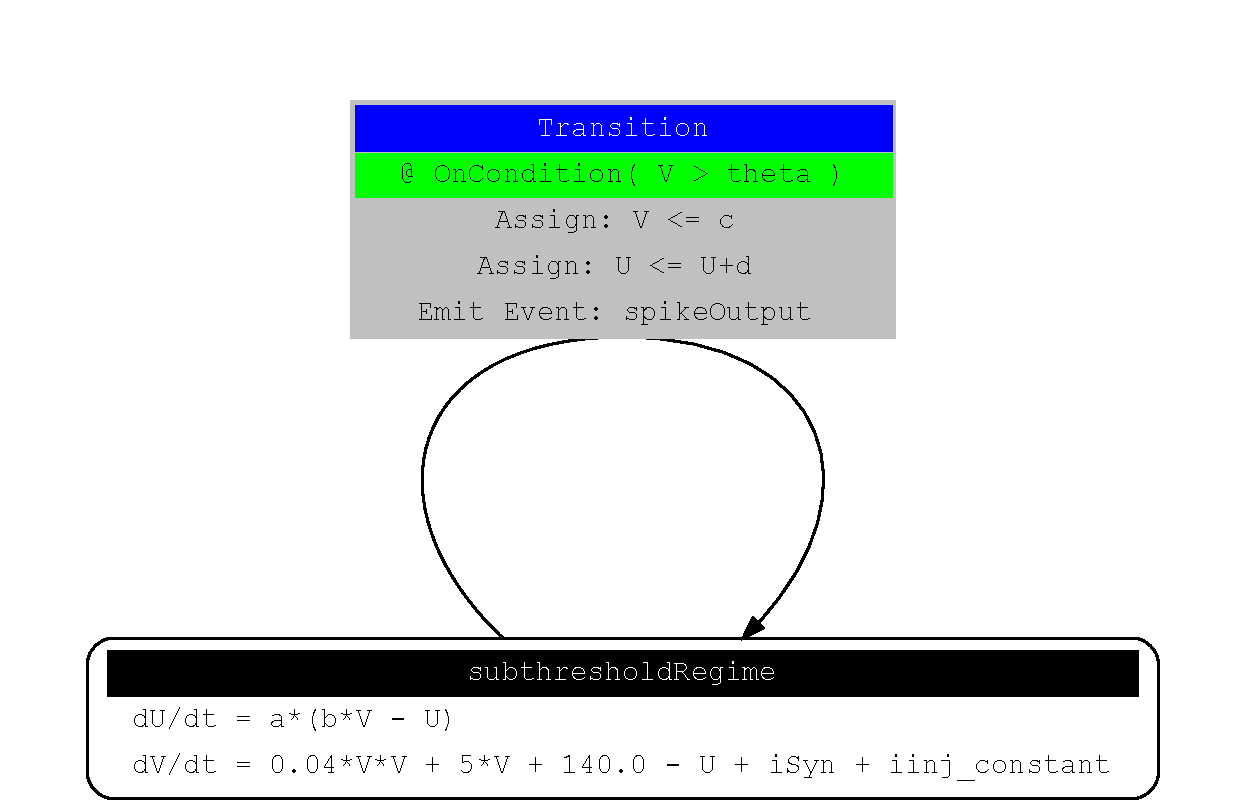
\includegraphics[width=8cm]{figures/example_IzRegimeTransGraph.pdf}
\protect\caption{{\tt RegimeGraph} for the XML model in this section.}
\label{fig:EX3_RegimeGraph}
\end{figure}

\noindent
Using this Abstraction Layer definition, as well as suitable parameters from the
user layer; $a=0.02, b=0.2, c=-65, d= 8, iinj\_constant= 5.0$, we can simulate
this, giving output as shown in Figure~\ref{fig:Ex1_Output}.

In Figure~\ref{fig:Ex1_Output}, we can see the value of the \StateVariable $V$
over time. We can also see that when the value of $V>theta$ triggers the
condition, we emit a spike, and the \StateAssignment of $V \leftarrow c$ resets
the value of $V$.
%
\noindent
The corresponding Abstraction Layer XML description for this model is the following:
%
\begin{lstlisting}

<?xml version='1.0' encoding='UTF-8'?>
<NineML xmlns="http://nineml.org/9ML/0.1">
    xmlns:xsi="http://www.w3.org/2001/XMLSchema-instance"
    xsi:schemaLocation="http://nineml.org/9ML/0.1 NineML\_v0.2.xsd">

  <ComponentClass name="izhikevichCellNew">

    <Parameter name="a" dimension="none"/>
    <Parameter name="c" dimension="voltage"/>
    <Parameter name="b" dimension="per_time"/>
    <Parameter name="d" dimension="voltage_per_time"/>
    <Parameter name="theta" dimension="voltage"/>

    <AnalogPort name="iSyn" mode="reduce" reduce_op="+" dimension="current"/>
    <AnalogPort name="U" mode="send" dimension="none"/>
    <AnalogPort name="V" mode="send" dimension="voltage"/>
    <EventPort name="spikeOutput" mode="send"/>


    <Dynamics>

        <StateVariable name="V" dimension="voltage"/>
        <StateVariable name="U" dimension="voltage_per_time"/>

        <Alias name="rv" dimension="none">
            <MathInline>V*U</MathInline>
        </Alias>

        <Regime name="subthresholdRegime">

          <TimeDerivative variable="U">
            <MathInline>a*(b*V - U)</MathInline>
          </TimeDerivative>

          <TimeDerivative variable="V">
            <MathInline>0.04*V*V + 5*V + 140.0 - U + iSyn</MathInline>
          </TimeDerivative>


          <OnCondition>
            <Trigger>
              <MathInline>V \&gt; theta </MathInline>
            </Trigger>

            <StateAssignment variable="V" >
              <MathInline>c</MathInline>
            </StateAssignment>

            <StateAssignment variable="U" >
              <MathInline>U+d</MathInline>
            </StateAssignment>

            <EventOut port="spikeOutput" />

          </OnCondition>

        </Regime>
    </Dynamics>

  </ComponentClass>
</NineML>
\end{lstlisting}

User Layer description for the above example:

\begin{lstlisting}
<?xml version='1.0' encoding='UTF-8'?>
<nineml xmlns="http://www.NineML.org/9ML/1.0" name="Izhikevich neuron">
  <import language="NineML">
    http://www.NineML.org/1.0/dimensions.9ml
  </import>
  <component name="Izhikevich neuron">
    <definition language="NineML">
      http://www.NineML.org/neurons/izhikevichCellNew.9ml
    </definition>
    <property name="V">
       <quantity>
         <value>
           <scalar>-60</scalar>
           <unit>mV</unit>
         </value>
       </quantity>
       <note><String>Initial value</String></note>
    </property>
    <property name="U">
       <quantity>
         <value>
           <scalar>0</scalar>
           <unit>mV_per_ms</unit>
         </value>
       </quantity>
       <note><String>Initial value</String></note>
    </property>
    <property name="theta">
       <quantity>
         <value>
           <scalar>50</scalar>
           <unit>mV</unit>
         </value>
       </quantity>
       <note><String>Parameter value (spike amplitude)</String></note>
    </property>
    <property name="a">
       <quantity>
         <value>
           <scalar>0.02</scalar>
           <unit>none</unit>
         </value>
       </quantity>
       <note><String>Parameter value</String></note>
    </property>
    <property name="b">
       <quantity>
         <value>
           <scalar>0.2</scalar>
           <unit>per_ms</unit>
         </value>
       </quantity>
       <note><String>Parameter value</String></note>
    </property>
    <property name="c">
       <quantity>
         <value>
           <scalar>-65</scalar>
           <unit>mV</unit>
         </value>
       </quantity>
       <note><String>Parameter value (reset voltage)</String></note>
    </property>
    <property name="d">
       <quantity>
         <value>
           <scalar>8</scalar>
           <unit>mV_per_ms</unit>
         </value>
       </quantity>
       <note><String>Parameter value</String></note>
    </property>
  </component>
</nineml>
\end{lstlisting}

Here, we show the simulation results of this XML representation.
\begin{figure}[htb!]
\center
%\includegraphics[width=14cm]{al/ParallelisingTransitions.pdf}example_IzRegimeTransGraph.pdf
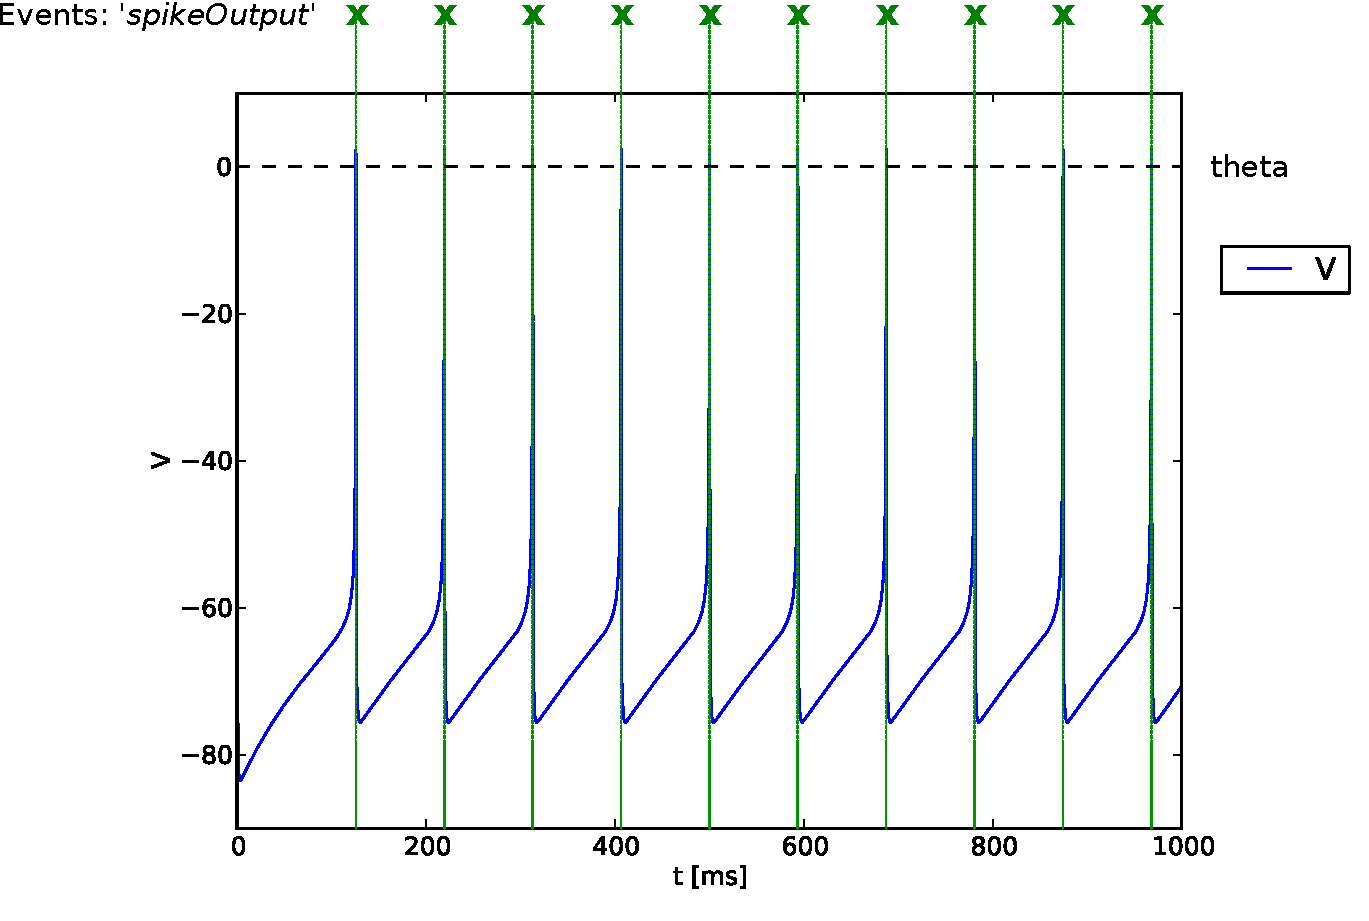
\includegraphics[width=8cm]{figures/example_IzVoltageWave.pdf}
\protect\caption{Result of simulating of the XML model in
this section}
\label{fig:Ex1_Output}
\end{figure}

\newpage
\subsection{Second XML example}

In this example, we build a representation of a integrate-and-fire neuron, with
an attached input synapse.
\noindent
We have a single \StateVariable, $iaf\_V$.
This time, the neuron has an absolute refractory period; which is implemented
by using 2 regimes. $RegularRegime$ \& $RefractoryRegime$
In $RegularRegime$, the neuron voltage evolves as:
\begin{eqnarray}
\frac{d(iaf\_V)}{dt} = \frac{ iaf\_gl*( iaf\_vrest - iaf\_V ) + iaf\_ISyn+cobaExcit\_I} {iaf\_cm}
\end{eqnarray}
In $RefractoryRegime$, the neuron voltage does not change in response to any
input:

\begin{eqnarray}
\frac{d(iaf\_V)}{dt} = 0
\end{eqnarray}
\noindent
In both Regimes, the synapses dynamics evolve as:
\begin{eqnarray}
\frac{d(cobaExcit\_g)}{dt} = - \frac{cobaExcit\_g}{cobaExcit\_tau}
\end{eqnarray}
\noindent
The neuron has 2 \EventPorts, $iaf\_spikeoutput$ is a send port, which sends
events when the neuron fires, and $cobaExcit\_spikeinput$ is a recv port,
which tells the attached synapse that it should `fire'.
\noindent
The neuron has 4 \Transitions, 2 \OnEvents  and 2 \OnConditions.
Two of the Transitions are triggered by $cobaExcit\_spikeinput$ events, which
cause the conductance of the synapse to increase by an amount $q$, These
happen in both Regimes.
The other \OnConditions:
\begin{itemize}
\item One is triggered the voltage being above threshold, which moves the
component from $RegularRegime$ to $RefractoryRegime$, sets V to the
reset-voltage also emits a spike
\item The other is triggered by enough time having passed for the component
to come out of the $RefractoryRegime$ and move back to the $RegularRegime$
\end{itemize}

The corresponding Regime Graph is shown in Figure 5.

\begin{figure}[htb!]
\center
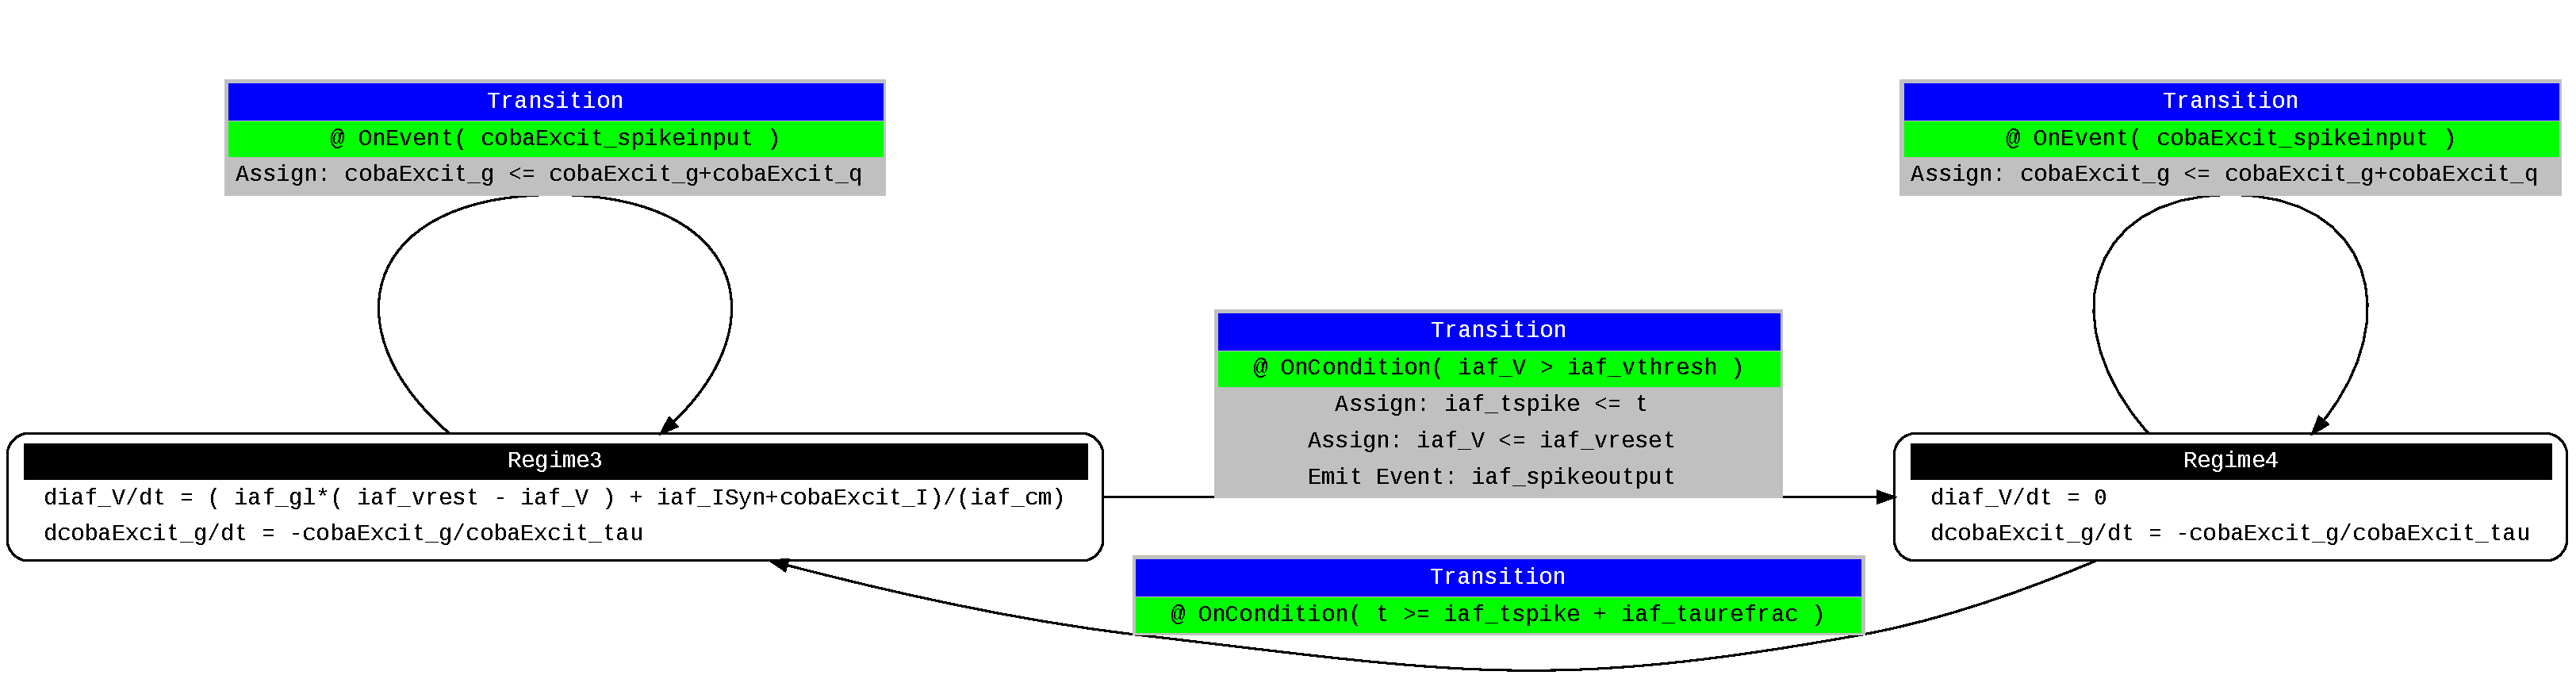
\includegraphics[width=14cm]{figures/demo2_Coba1_trnasition.pdf}
\protect\caption{RegimeGraph for the XML model in this section}
\label{fig:EX2_trans}
\end{figure}

The resulting XML description for the Abstraction Layer is :

\begin{lstlisting}[label=code:xmliaf2]
<?xml version='1.0' encoding='UTF-8'?>
<NineML xmlns="http://nineml.org/9ML/0.1">
  <ComponentClass name="iaf_1coba">
    <AnalogPort mode="send" name="iaf_V"/>
    <AnalogPort mode="reduce" reduce_op="+" name="iaf_ISyn"/>
    <AnalogPort mode="send" name="cobaExcit_I"/>
    <EventPort mode="send" name="iaf_spikeoutput"/>
    <EventPort mode="recv" name="cobaExcit_spikeinput"/>
    <Parameter dimension="area" name="iaf_cm"/>
    <Parameter dimension="time" name="iaf_taurefrac"/>
    <Parameter dimension="conductance" name="iaf_gl"/>
    <Parameter dimension="voltage" name="iaf_vreset"/>
    <Parameter dimension="voltage" name="iaf_vrest"/>
    <Parameter dimension="voltage" name="iaf_vthresh"/>
    <Parameter dimension="time" name="cobaExcit_tau"/>
    <Parameter dimension="conductance" name="cobaExcit_q"/>
    <Parameter dimension="voltage" name="cobaExcit_vrev"/>
    <Dynamics>
      <Regime name="RefractoryRegime">
        <TimeDerivative variable="iaf_V">
          <MathInline>0</MathInline>
        </TimeDerivative>
        <TimeDerivative variable="cobaExcit_g">
          <MathInline>-cobaExcit_g/cobaExcit_tau</MathInline>
        </TimeDerivative>
        <OnEvent target_regime="RefractoryRegime" src_port="cobaExcit_spikeinput">
          <StateAssignment variable="cobaExcit_g">
            <MathInline>cobaExcit_g+cobaExcit_q</MathInline>
          </StateAssignment>
        </OnEvent>
        <OnCondition target_regime="RegularRegime">
          <Trigger>
            <MathInline>t &gt;= iaf_tspike + iaf_taurefrac</MathInline>
          </Trigger>
        </OnCondition>
      </Regime>
      <Regime name="RegularRegime">
        <TimeDerivative variable="iaf_V">
          <MathInline>( iaf_gl*( iaf_vrest - iaf_V ) + iaf_ISyn+cobaExcit_I)/(iaf_cm)</MathInline>
        </TimeDerivative>
        <TimeDerivative variable="cobaExcit_g">
          <MathInline>-cobaExcit_g/cobaExcit_tau</MathInline>
        </TimeDerivative>
        <OnEvent target_regime="RegularRegime" src_port="cobaExcit_spikeinput">
          <StateAssignment variable="cobaExcit_g">
            <MathInline>cobaExcit_g+cobaExcit_q</MathInline>
          </StateAssignment>
        </OnEvent>
        <OnCondition target_regime="RefractoryRegime">
          <StateAssignment variable="iaf_tspike">
            <MathInline>t</MathInline>
          </StateAssignment>
          <StateAssignment variable="iaf_V">
            <MathInline>iaf_vreset</MathInline>
          </StateAssignment>
          <EventOut port="iaf_spikeoutput"/>
          <Trigger>
            <MathInline>iaf_V &gt; iaf_vthresh</MathInline>
          </Trigger>
        </OnCondition>
      </Regime>
      <Alias name="cobaExcit_I">
        <MathInline>cobaExcit_g*(cobaExcit_vrev-iaf_V)</MathInline>
      </Alias>
      <StateVariable dimension="voltage" name="iaf_V"/>
      <StateVariable dimension="time" name="iaf_tspike"/>
      <StateVariable dimension="conductance" name="cobaExcit_g"/>
    </Dynamics>
  </ComponentClass>
</NineML>

\end{lstlisting}

User Layer description for the above example:

\begin{lstlisting}
<?xml version='1.0' encoding='UTF-8'?>
<nineml xmlns="http://www.NineML.org/9ML/1.0" name="IaF neuron with synapse">
  <import language="NineML">
    http://www.NineML.org/1.0/dimensions.9ml
  </import>
  <component name="IaF neuron">
    <definition language="NineML">
      http://www.NineML.org/neurons/iaf_1coba.9ml
    </definition>
    <property name="iaf_V">
       <quantity>
         <value>
           <scalar>-60</scalar>
           <unit>mV</unit>
         </value>
       </quantity>
       <note><String>Initial value</String></note>
    </property>
    <property name="iaf_tspike">
       <quantity>
         <value>
           <scalar>-1</scalar>
           <unit>ms</unit>
         </value>
       </quantity>
       <note><String>Initial value</String></note>
    </property>
    <property name="cobaExcit_g">
       <quantity>
         <value>
           <scalar>0</scalar>
           <unit>mS</unit>
         </value>
       </quantity>
       <note><String>Initial value</String></note>
    </property>
    <property name="iaf_cm">
       <quantity>
         <value>
           <scalar>0.02</scalar>
           <unit>cm_square</unit>
         </value>
       </quantity>
       <note><String>Parameter value</String></note>
    </property>
    <property name="iaf_taurefrac">
       <quantity>
         <value>
           <scalar>3</scalar>
           <unit>ms</unit>
         </value>
       </quantity>
       <note><String>Parameter value (refractory period)</String></note>
    </property>
    <property name="iaf_gl">
       <quantity>
         <value>
           <scalar>0.1</scalar>
           <unit>mS</unit>
         </value>
       </quantity>
       <note><String>Parameter value (leak conductance)</String></note>
    </property>
    <property name="iaf_vreset">
       <quantity>
         <value>
           <scalar>-70</scalar>
           <unit>mV</unit>
         </value>
       </quantity>
       <note><String>Parameter value (reset voltage)</String></note>
    </property>
    <property name="iaf_vrest">
       <quantity>
         <value>
           <scalar>-60</scalar>
           <unit>mV</unit>
         </value>
       </quantity>
       <note><String>Parameter value (resting potential)</String></note>
    </property>
    <property name="iaf_vthresh">
       <quantity>
         <value>
           <scalar>20</scalar>
           <unit>mV</unit>
         </value>
       </quantity>
       <note><String>Parameter value (threshold potential)</String></note>
    </property>
    <property name="cobaExcit_tau">
       <quantity>
         <value>
           <scalar>2</scalar>
           <unit>ms</unit>
         </value>
       </quantity>
       <note><String>Parameter value (synaptic time constant)</String></note>
    </property>
    <property name="cobaExcit_q">
       <quantity>
         <value>
           <scalar>1</scalar>
           <unit>ms</unit>
         </value>
       </quantity>
       <note><String>Parameter value (conductance increase on spike)</String></note>
    </property>
    <property name="cobaExcit_vrev">
       <quantity>
         <value>
           <scalar>0</scalar>
           <unit>mV</unit>
         </value>
       </quantity>
       <note><String>Parameter value (synaptic reversal potential)</String></note>
    </property>
  </component>
</nineml>
\end{lstlisting}

The simulation results is presented in Figure 6.
\begin{figure}[htb!]
\center
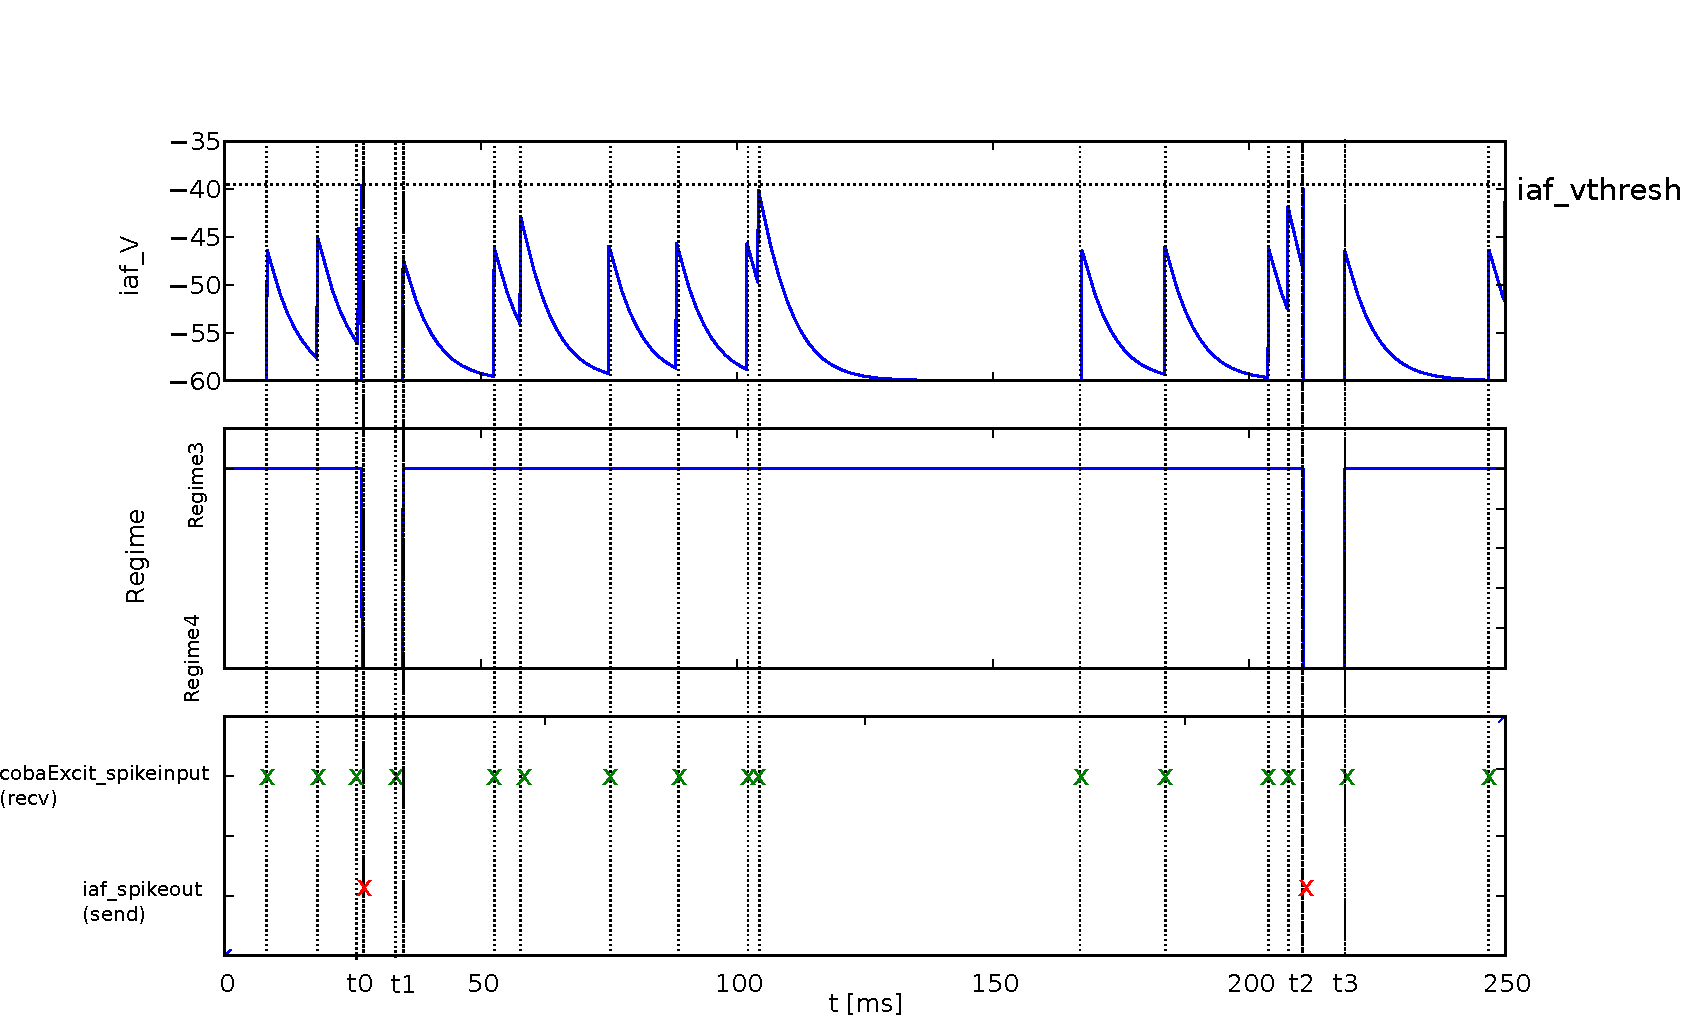
\includegraphics[width=14cm]{figures/demo2_Coba1_out.pdf}
\protect\caption{Result of simulating of the XML model in this section.
$cobaExcit\_spikeinput$ is fed events from an external Poisson generator
in this simulation}
\label{fig:EX2_Output}
\end{figure}

\pagebreak

\newpage

\section{Transition Resolution}
\label{resolution}

This section outlines pseudo code which defines the order of
\Transition-triggering, state assignment execution, event emission,
transmission and resolution in a system of connected components.
Implementations do not need to implement this algorithm but should produce
the same behaviours.

A {\tt TransitionResolutionBlock} represents an instant in time. It begins
before any \Transitions occur and ends after each component has moved
into its new \Regime, all \textbf{StateAssignments} have been executed
and all \Events generated and resolved in the system.

\subsection{Serial Implementation of Transition Resolution}

\newcommand{\CN}[0]{\textsl{C\_n}}

We have a system of \textsl{N} components \textsl{\{C\_1,C\_2,...,C\_N\}},
at time, \textsl{t}, where each component, \CN, is in \Regime
$R^{t}_{n}$.

\noindent From \Regime $R^{t}_{n}$, there are:
\begin{itemize}
\item OnEvent \Transitions $OnEv^{t}_{n} = \{ ... \}$
\item OnCondition \Transitions $OnCond^{t}_{n} = \{ ... \}$
\end{itemize}

\newcommand{\send}[0]{\texttt{send} }
\newcommand{\recv}[0]{\texttt{recv} }

\noindent Component \CN
has:
\begin{itemize}
\item \send EventPorts \textsl{EvSend = \{$EvSend_{n,1,}$, $EvSend_{n,2,}$, ... \}}
\item \recv EventPorts \textsl{EvRecv = \{$EvRecv_{n,1,}$, $EvRecv_{n,2,}$, ... \}}
\end{itemize}

\noindent \EventPort connections are stored in a a map,
\textsl{EvPortConnections}, which maps EvSend to a list of EvRecv ports. i.e.,

\textsl{\{EvSend $\rightarrow$ [EvRecv,EvRecv,..,EvRecv], EvSend $\rightarrow$
[EvRecv,EvRecv,EvRecv,...,EvRecv]\}}.

\newcommand{\RCLn}{$RCL_n$}
\newcommand{\AUTQn}{$AUTQ_n$}
\newcommand{\EQn}{$EQ_n$}

\noindent Each component has 3 associated data structures
\begin{itemize}
\item RegimeChangeList (\RCLn) (This list will contain target-regimes of
triggered transitions)
\item ActiveUnresolvedTransitionsQueue (\AUTQn) (This queue will
contain transitions which will occur, but their effects have not be
evaluated yet)
\item EventQueue (\EQn) (This list contains events delivered to this
component from other components via EventPort-connections)
\end{itemize}

\subsubsection{Algorithm}

\begin{enumerate}
\item Enter {\tt TransitionResolutionBlock}
\item For each component, \CN: clear \RCLn, \AUTQn and \EQn.
\item For each component, \CN: for each \textsl{oncond} in $OnCond^{t}_{n}$ : if
\textsl{oncond.trigger} evaluates to true, add \textsl{oncond} to \AUTQn.
\item For each component, \CN:  for each \textsl{tr} in \AUTQn :
\begin{itemize}
\item
remove \textsl{tr} from \AUTQn
\item add the target\_regime to \RCLn
\item for each
\textsl{action} in \textsl{tr.do}:
\begin{itemize}
\item if \textsl{action} is an OutputEvent: test
if the OutputEvent port is a key in \textsl{EvPortConnections}. If so, add the
    OutputEvent to the EventQueue (\textsl{EQ\_{target}}) corresponding to each
    \textsl{EvRecv} in the \textsl{EvPortConnections} map.

\item  if \textsl{action}  is a StateAssignment, execute that state-assignment
immediately.
\end{itemize}
\end{itemize}

\item For each component \CN: for each event, \textsl{EvRecv} in \EQn: test
whether there is a transition, \textsl{tr} triggered by this event, i.e an
OnEvent in $OnEv^t_n$ from $R^t_n$ ; if so; then add it to \AUTQn.

\item While any component has a non-empty \textsl{AUTQ}: Goto (4).

\item For each component, \CN, check that all the target-regimes in the \RCLn
are the same regime. (If not raise a RuntimeError). Each component moves into
this target-regime, or remains in the same regime if \RCLn is empty.

\item Leave {\tt TransitionResolutionBlock}

\end{enumerate}

\subsubsection{Notes}

\begin{enumerate}
\item  There is no order defined in transitions; this means
that the order of resolution of state assignments can be ambiguous. If, for
example, we have two transitions, T1 and T2, originating from the same \Regime,
in which T1 contains the state assignment \textsl{V=V+1} and T2 contains the
assignment \textsl{V=V*V}, and both transitions are triggered, then there is no
guarantee about the value of V. It is up the user to ensure this does not
happen.

\item This Resolution System allows \emph{cascading} of Events, which in theory
could be recursive through components, depending on connectivity. The
implementation allows for this; and it is the users responsibility to ensure
that there are not such issues. The implementation may decided to terminate
Step (6) after a given number (say 1000) of iterations to prevent infinite
loops.

\item Flattening of hierarchical components; implementation should ensure that
the behaviour of a flattened component is identical to that of an unflattened
component.
\end{enumerate}

\subsection{Parallelising of Event Resolution}

This algorithm can be parallelised as following. We create a thread for each
Component, which can independently execute Steps (3 to 6). The threads need
to be synchronized after steps (4) and (5) as shown in
Figure~\ref{ParallelisingTransitions}.

\begin{figure}[htb!]
\center
\includegraphics[width=14cm]{images/ParallelisingTransitions.pdf}
\protect\caption{Parallelising of Event Resolution.}
\label{ParallelisingTransitions}
\end{figure}
\bibliographystyle{apalike}
%\bibliography{CondensedUL}

\end{document}

